Throughout project development, several datasets from various sources have been used to fulfil Magpie's project goal. Below is an overview of Magpie's data stack:
\begin{figure}[h!]
    \centering
    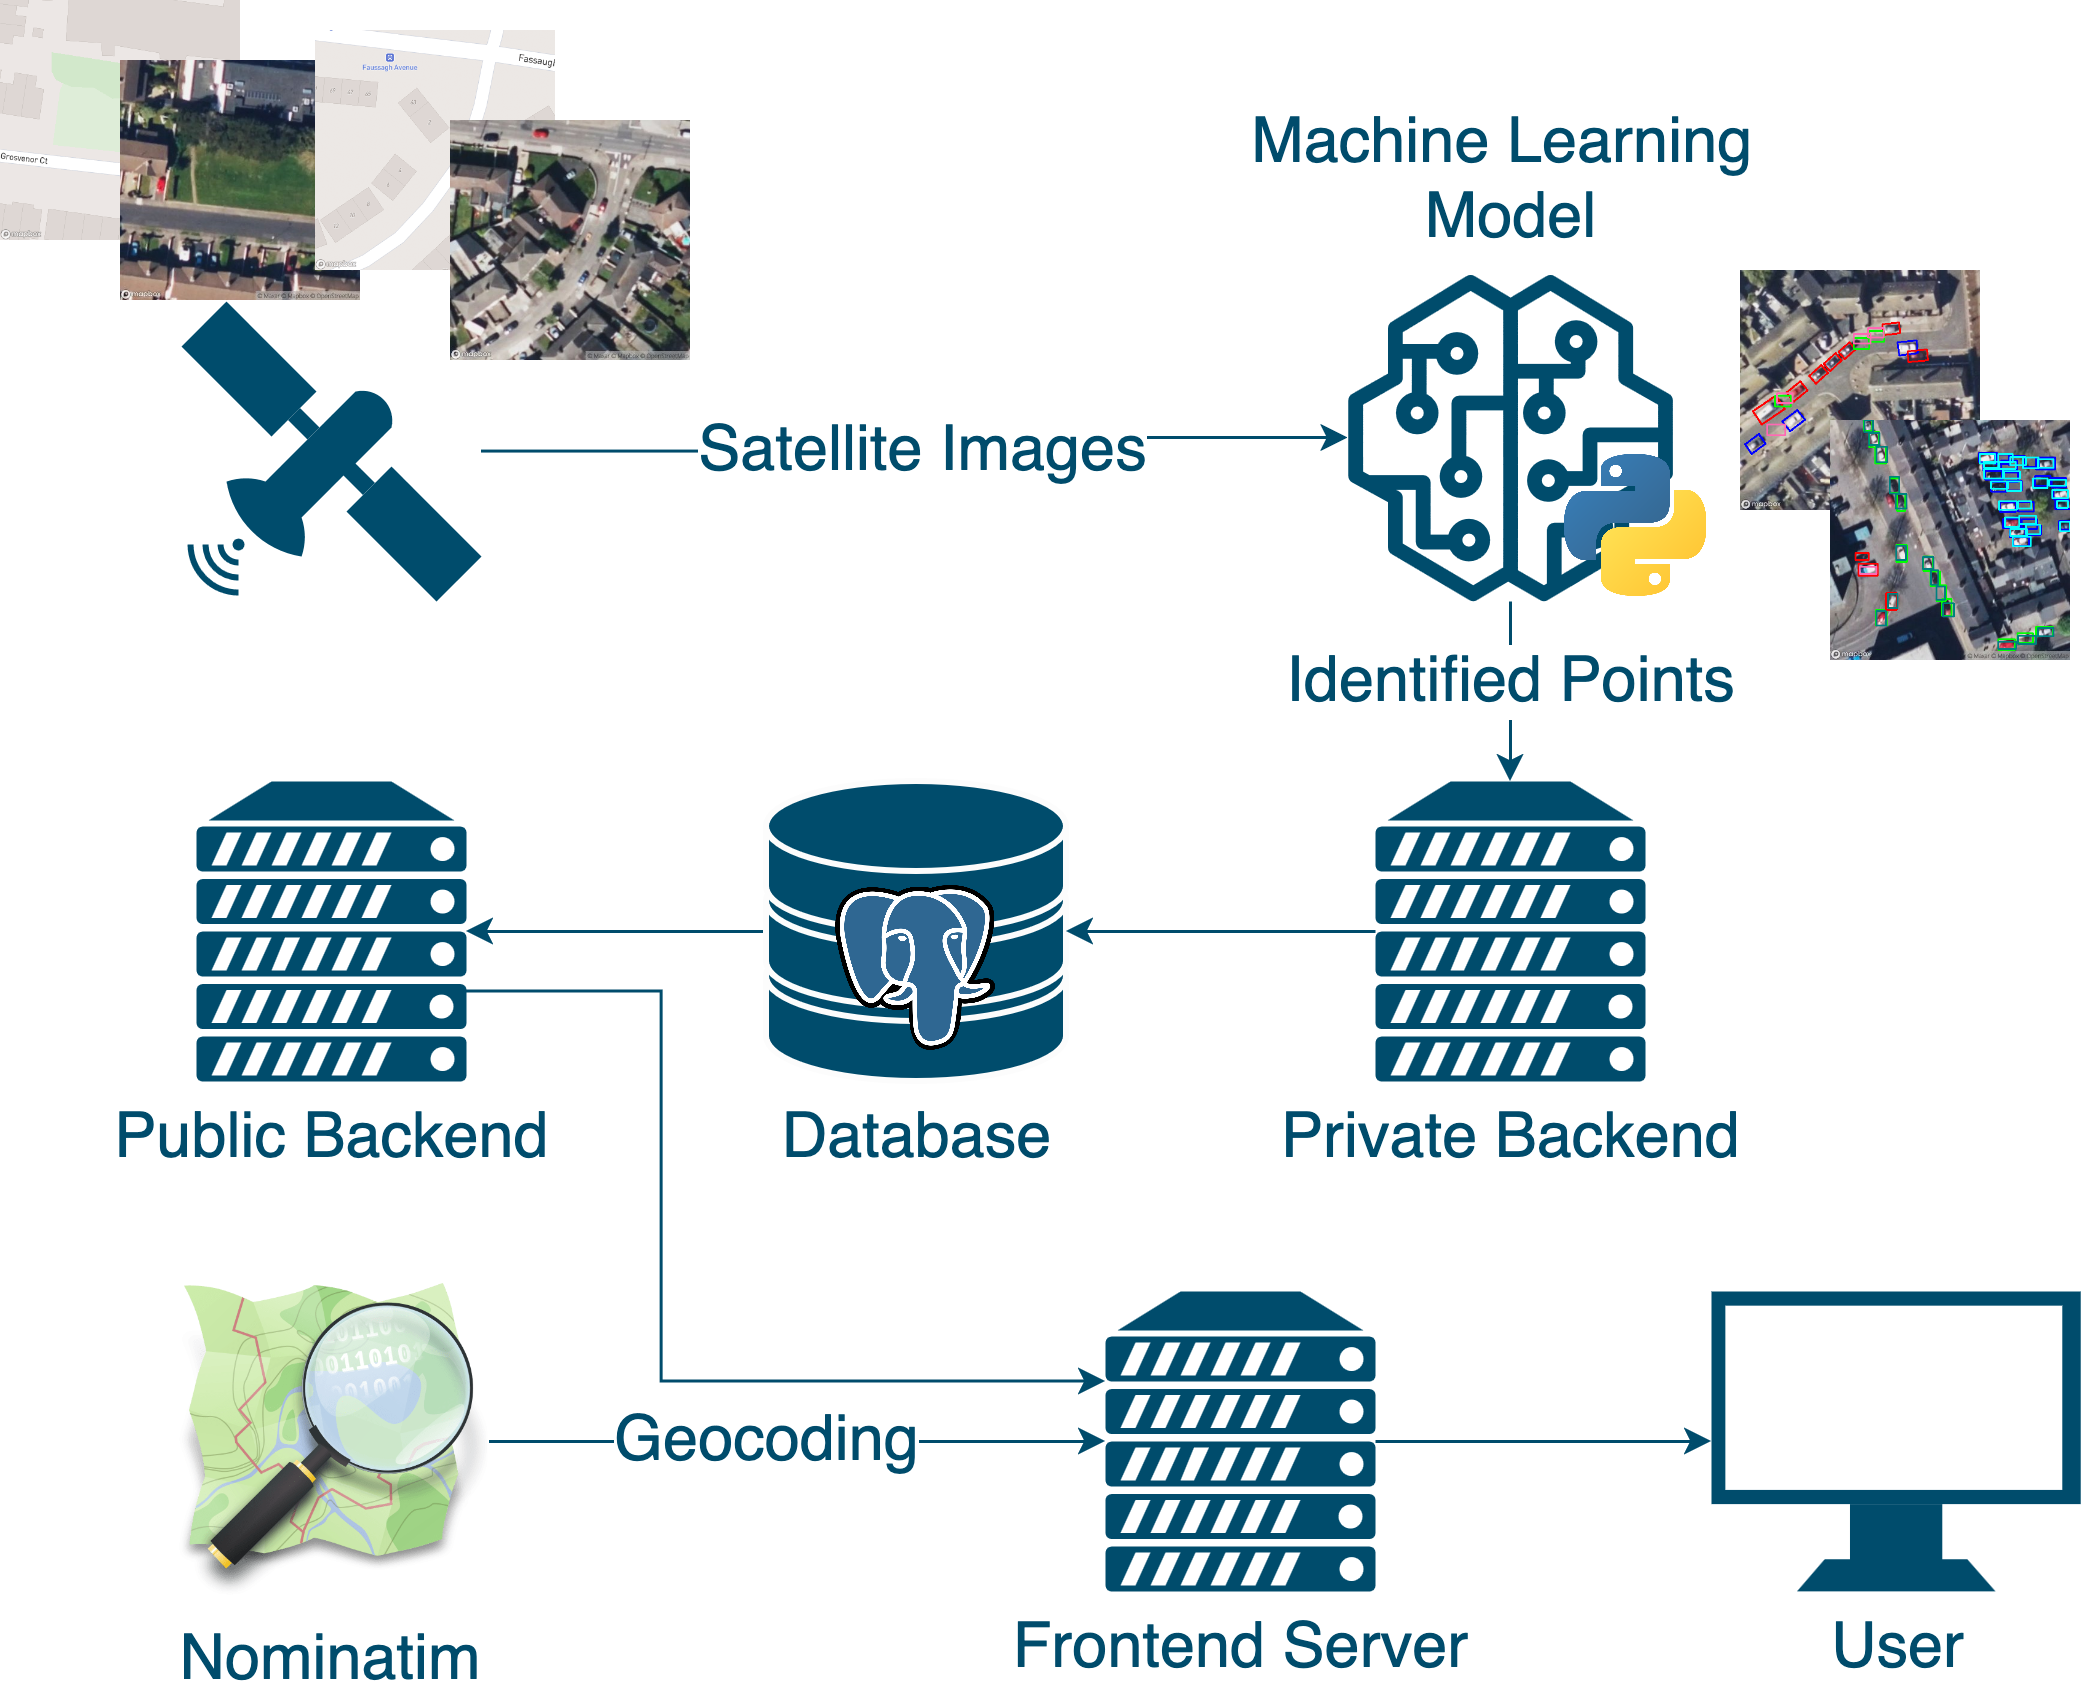
\includegraphics[width=0.7\textwidth]{images/magpie-data-stack.png}
    \caption{Magpie Data Stack}
\end{figure}\\

\subsubsection{Data sourcing \& Collection}
Three main categories of data have been sourced for Magpie:
\begin{enumerate}
    \item For the \emph{Machine learning models}
    \item For the \emph{Amenity data}
    \item For the \emph{Search functionality}
\end{enumerate}

\textbf{1.1 Machine learning models - Car detection}\\
The Mapbox Static Images API was used to retrieve all the images used for the machine learning models of this project.

First, 250 images were downloaded using CSV data from the following sources:
\begin{itemize}
    \item \textbf{Data.gov.ie}: Online portal containing thousands of publicly available datasets about Ireland
    \item \textbf{Smart Dublin}: Founded by Dublin local authorities, their goal is to look for innovative technological solutions for local environmental, social, mobility, government and living issues. They also have hundreds of publicly available datasets
    \item \textbf{Kaggle}: a data science and machine learning platform part of Google Cloud where competitions are hosted, in addition to thousands of publicly available datasets
\end{itemize}
These CSV files contained information on the location of certain facilities such as rentals, coach parking, public parks. This location was latitude and longitude which we needed to input into the script to download images, as well as the street name of that location which was used to name the downloaded image.\\

\begin{listing}[h!]
    \centering
    \caption{Python script to obtain training images for ML model}
    \begin{minted}{python3}
        # CSV file containing location information
        df = pd.read_csv("2020-coach-parking-dcc-1.csv")
        location_data = df.to_dict('records')

        # function to download image using location information from CSV dataset
        def get_images(name, latitude, longitude):
            url = f'https://api.mapbox.com/styles/v1/mapbox/satellite-v9/static/{longitude},{latitude},18,0,0/400x400?access_token=pk.eyJ1Ijoia2F1c3R1Ymh0cml2ZWRpIiwiYSI6ImNtMWo2NndsbzB4N3EycHM1aGF2cDd5NzkifQ.4aegzX6Kfy3zW8pHkLWU7Q'
            response = requests.get(url)
            print(response)
            if response.status_code == 200:
                img = Image.open(BytesIO(response.content))
                if not os.path.exists('output'):
                    os.makedirs('output')

                output_folder = 'output'
                output_path = os.path.join(output_folder, f'{name}_coach_parking.png')
                img.save(output_path)
                print(f"Image saved to {output_path}")

        # function to extract location \& name location from CSV dataset
        for place in location_data:
        name = place["Street Name"]
        if ("/" in name):
            name = name.replace("/", "-")
        latitude = place["Latitude"]
        longitude = place["Longitude"]
        get_images(name, latitude, longitude)
    \end{minted}
\end{listing}
Following successful model training and tuning, a further 19,536 satellite images were downloaded spanning Dublin City area illustrated in the figure below. The machine learning model was then applied to those images to detect the cars.
\begin{figure}[h!]
    \centering
    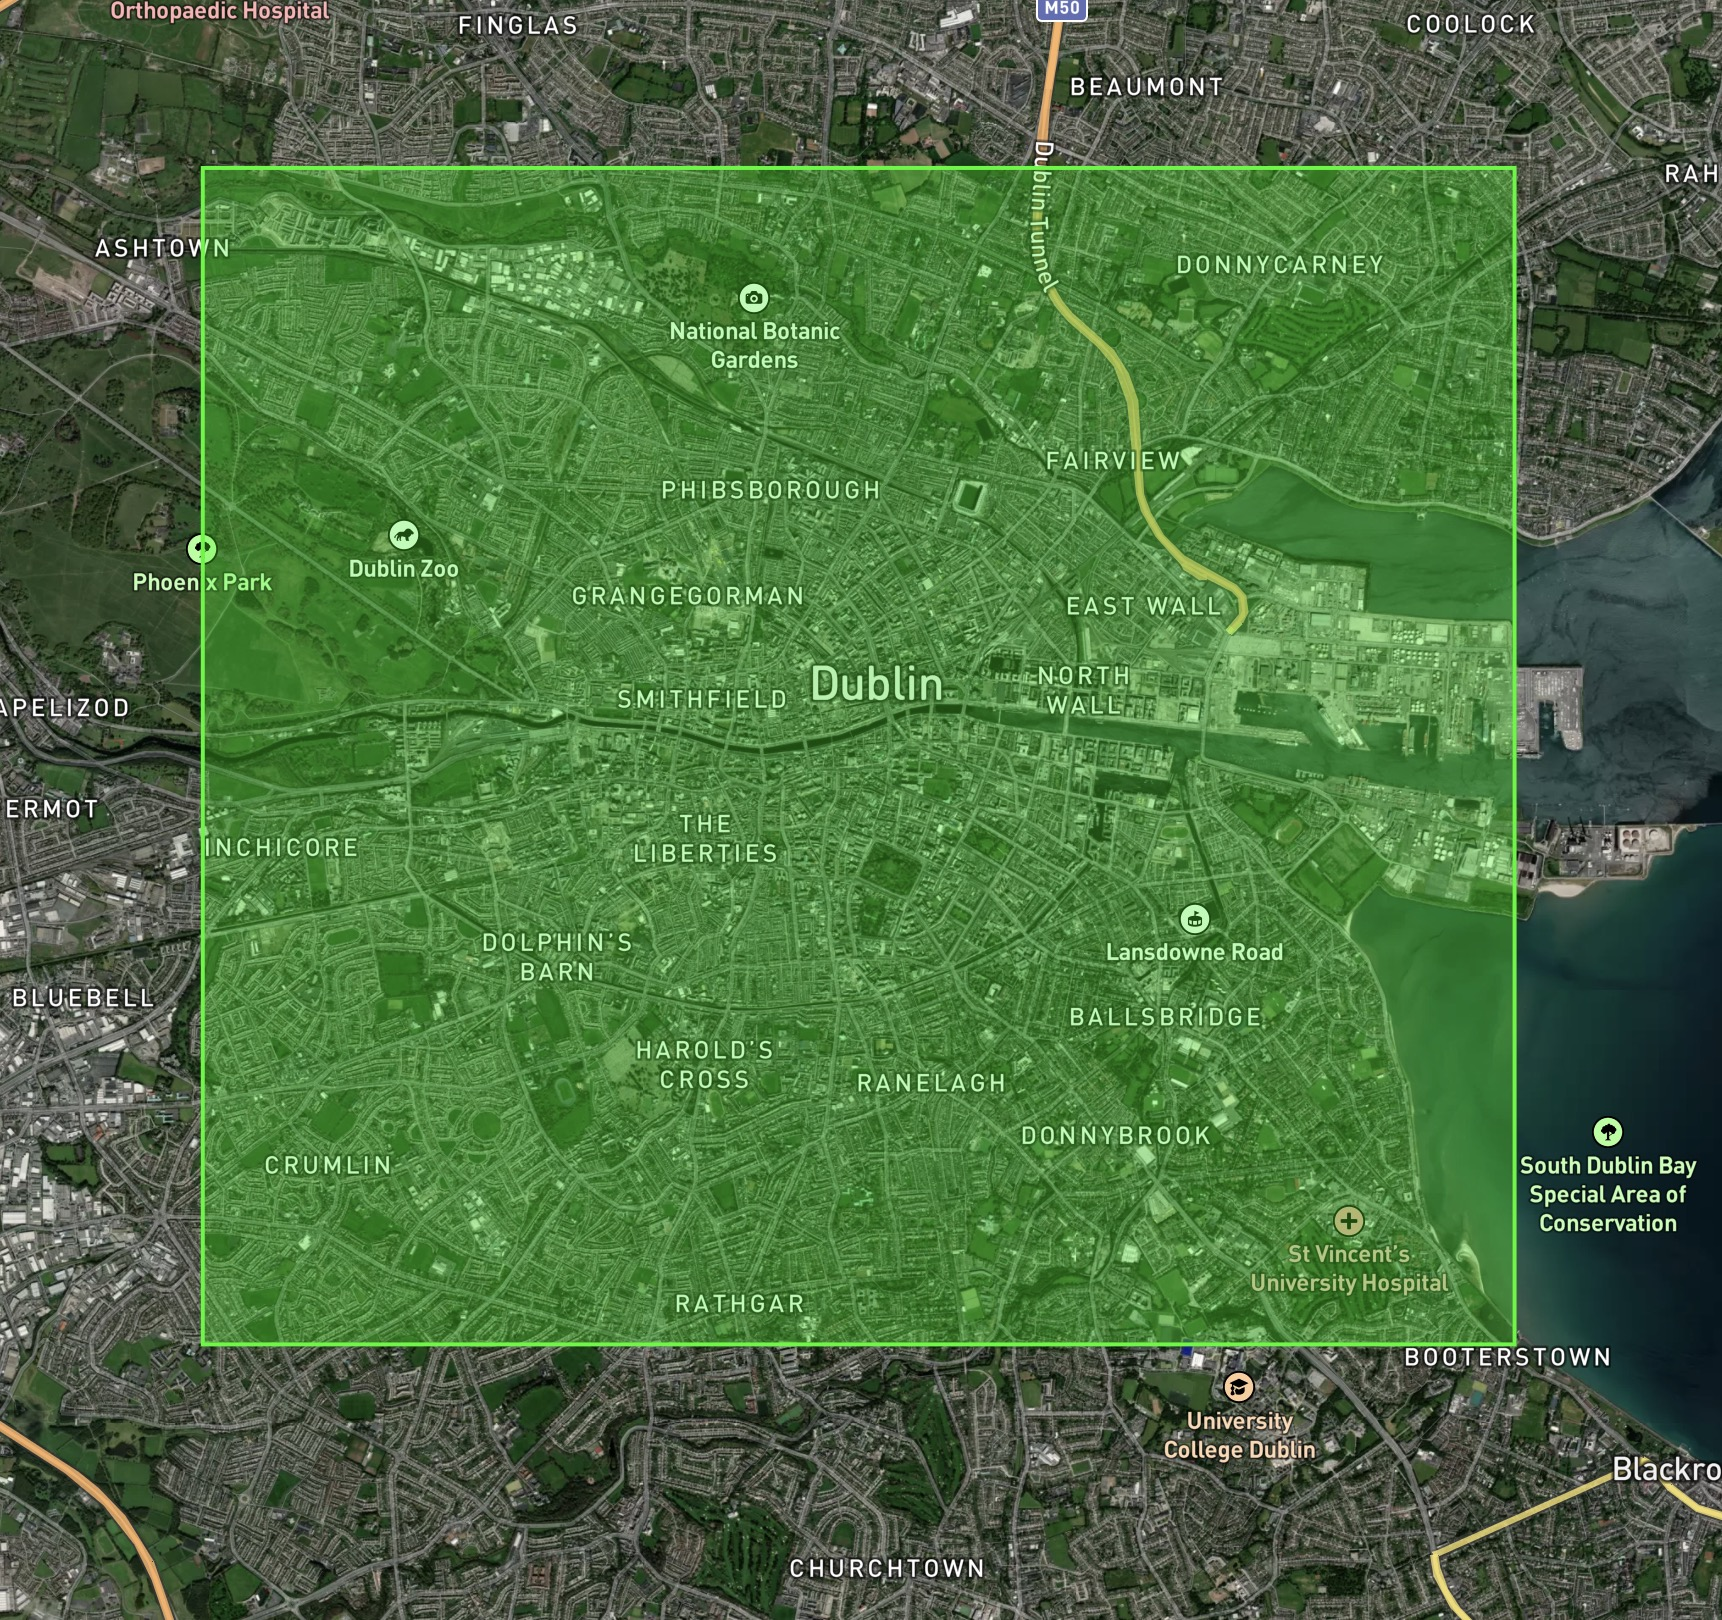
\includegraphics[width=0.6\textwidth]{images/dublin-img-area.jpg}
    \caption{Dublin Area Delimitation for Parking data}
\end{figure}\\

\textbf{1.2 Machine learning models - Parking detection}\\
An additional 19,536 map-view images corresponding to the satellite images used for car detection were downloaded using the MapBox API to create the custom mask used for detecting parked cars.\\
Our project has two main Python scripts, \texttt{parking\_detection.py} and\\ \texttt{parking\_detection\_local.py} to localize parking spots.\\
In \texttt{parking\_detection.py}, the satellite images (Mapbox Satellite) and corresponding road mask images (Mapbox Streets) are retrieved for a specific area contained within a bounding box, defined by its top-left and bottom-right coordinates, directly from the Mapbox API.\\ \\
From the coordinates of the specific bounding box, the center coordinates of all the images necessary to make up that area are calculated, and the images are then retrieved.
While in \texttt{parking\_detection\_local.py}, the original parking detection script is adapted to run on a database of locally stored Mapbox Satellite images and the corresponding Mapbox Streets images, covering the entirety of Dublin city.\\ \\

Extensive testing was done at all the different stages of development of the scripts to identify the optimal thresholds and parameters using test images from Mapbox, in a variety of scenarios including edge cases or cases prone to causing issues.\\

\textbf{2. Amenity data}\\
CSV files were collected from multiple sources mentioned above, notable Data.gov.ie and Smart Dublin. Below is a list relative to each amenity currently present on Magpie:
\begin{itemize}
    \item Parking meter = Data.gov.ie (link to appendix)
    \item Bike stand = Data.gov.ie (link to appendix)
    \item Public Wifi = Smart Dublin (link to appendix)
    \item Library = Smart Dublin (link to appendix)
    \item Multi-storey Car park = Data.gov.ie (link to appendix)
    \item Drinking water fountain = Data.gov.ie (link to appendix)
    \item Public toilet = Data.gov.ie (link to appendix)
    \item Bike sharing station = Data.gov.ie (link to appendix)
    \item Car parking = Novel ML technique
    \item Accessible parking = Data.gov.ie (link to appendix)
    \item Public bins = Smart Dublin (link to appendix)
    \item Coach parking = Data.gov.ie (link to appendix)
\end{itemize}
To complement this data visually on the map, we used SVG icons from \textbf{Icons8}, a UX design agency that provide high quality, free-to-use icons for personal and commercial web projects.\\

\textbf{3. Search functionality}\\
Nominatim is a geocoding solution created by the OpenStreetMap Foundation. Magpie uses a self-hosted instance of Nominatim for geocoding and reverse-geocoding tasks. Using the Nominatim API, the frontend server can request the coordinates associated with a place name. This is used in the search functionality of the frontend.

When the user saves a location, the frontend will also query Nominatim, but this
time with a set of coordinates. Nominatim will then return the closest place
name to the given coordinates, which is then sent to the database alongside the
location data.

\subsubsection{Data storage}
\textbf{Machine learning models data}\\
The 250 training images are stored locally.
The 19,536 satellite and 19,536 map-view images are also stored locally.

\textbf{Amenity points}\\
The CSV data obtained from sources named above are stored on the Postgres database server.\\
The amenity icons were downloaded locally then stored on the Magpie frontend server.

\textbf{Search functionality}\\
Any actions which involve data querying, requests and storage are handled by Nominatim, and therefore not stored on any of Magpie's servers.
